\documentclass{article}
\usepackage{graphicx} % Required for inserting images
\usepackage{float}
\usepackage{listings}
\usepackage{hyperref}
\hypersetup{
    colorlinks=true,    % use colors instead of boxes
    linkcolor=black,     % color for internal links (like references)
    citecolor=black,     % color for citations
    urlcolor=black       % color for URLs
}

\usepackage{fancyhdr}

\pagestyle{fancy}
\fancyhf{}
\rhead{\today}
\lhead{\bfseries PES2UG23CS032}
\rfoot{}
\cfoot{\thepage}

\title{DBMS Lab Submission}
\author{Aditya Hegde \@- PES2UG23CS032}
\date{\today}

\begin{document}

\maketitle

\section{Objective}

To learn and understand DDL statements while executing queries. To create a relational database from the provided ER diagram and Relational Schema

\section{Task 1}

As per the given Description, ER diagram, and Relational Schema \@– create the tables using DDL commands and add the required constraints.

\begin{figure}[H]
    \centering
    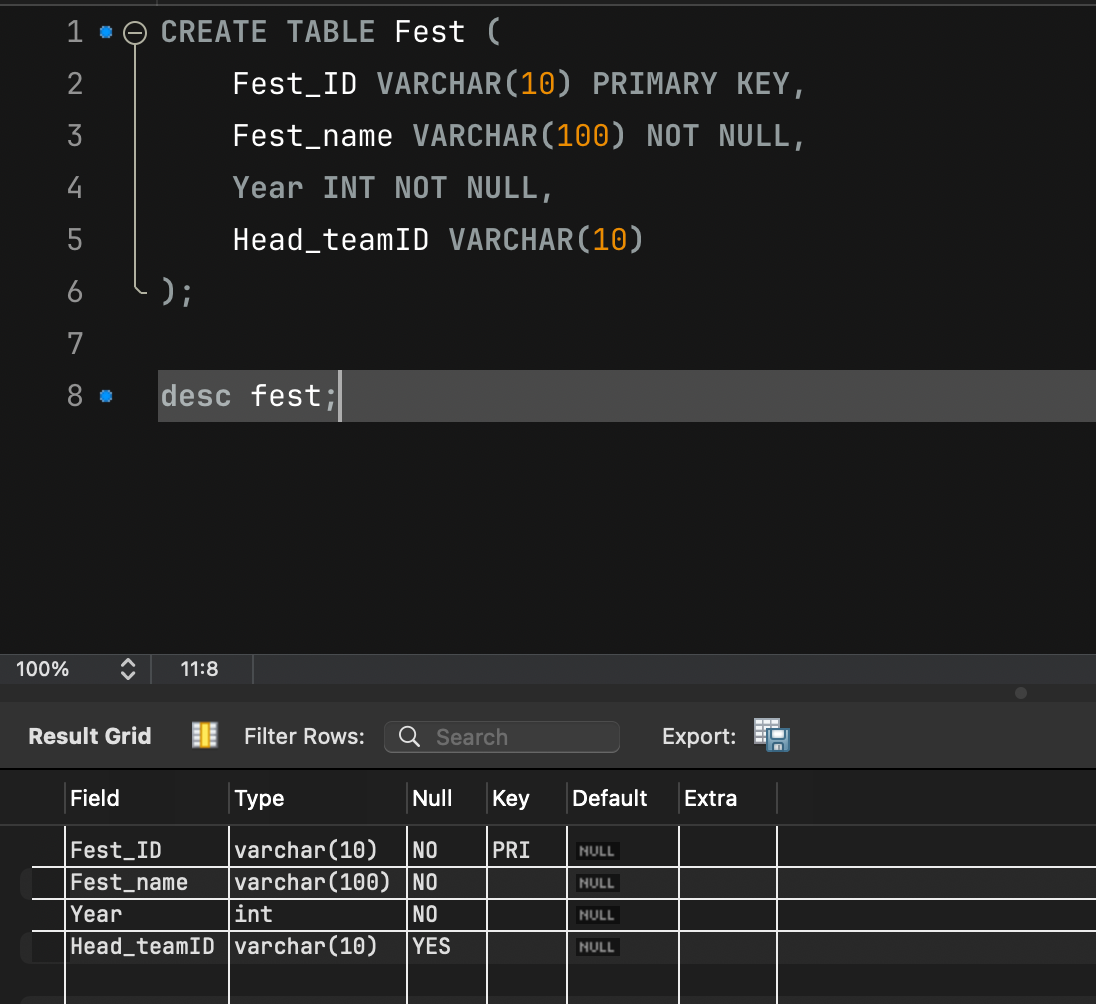
\includegraphics[width=0.7\linewidth]{images/task 1/1.png}
\end{figure}

\begin{figure}[H]
    \centering
    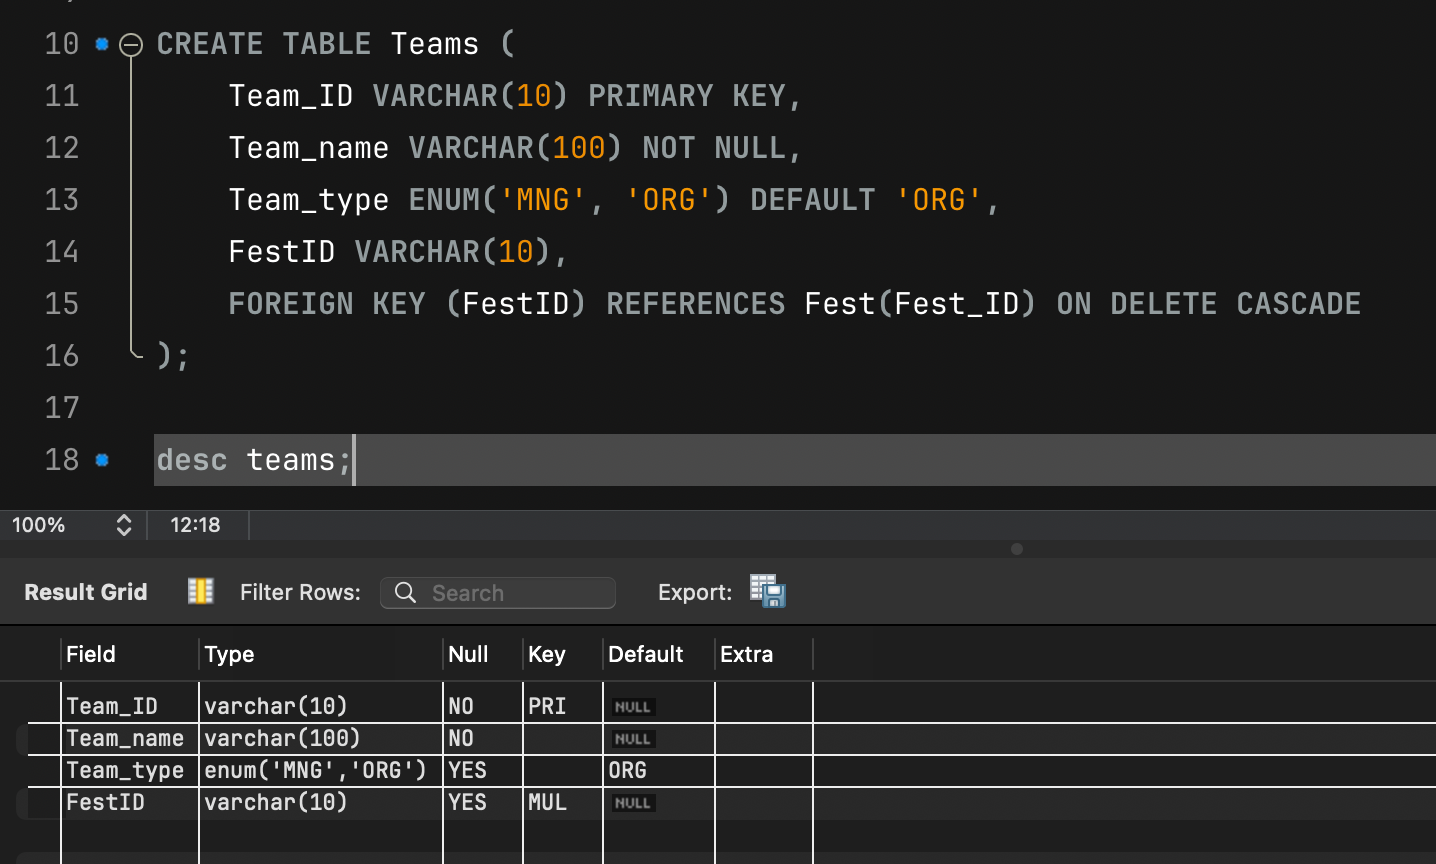
\includegraphics[width=0.7\linewidth]{images/task 1/2.png}
\end{figure}

\begin{figure}[H]
    \centering
    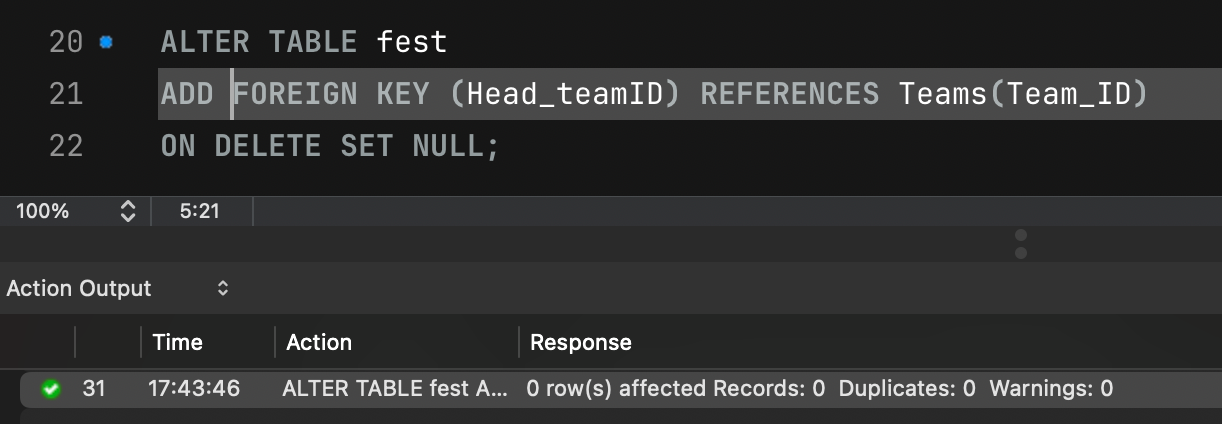
\includegraphics[width=0.7\linewidth]{images/task 1/3.png}
\end{figure}

\begin{figure}[H]
    \centering
    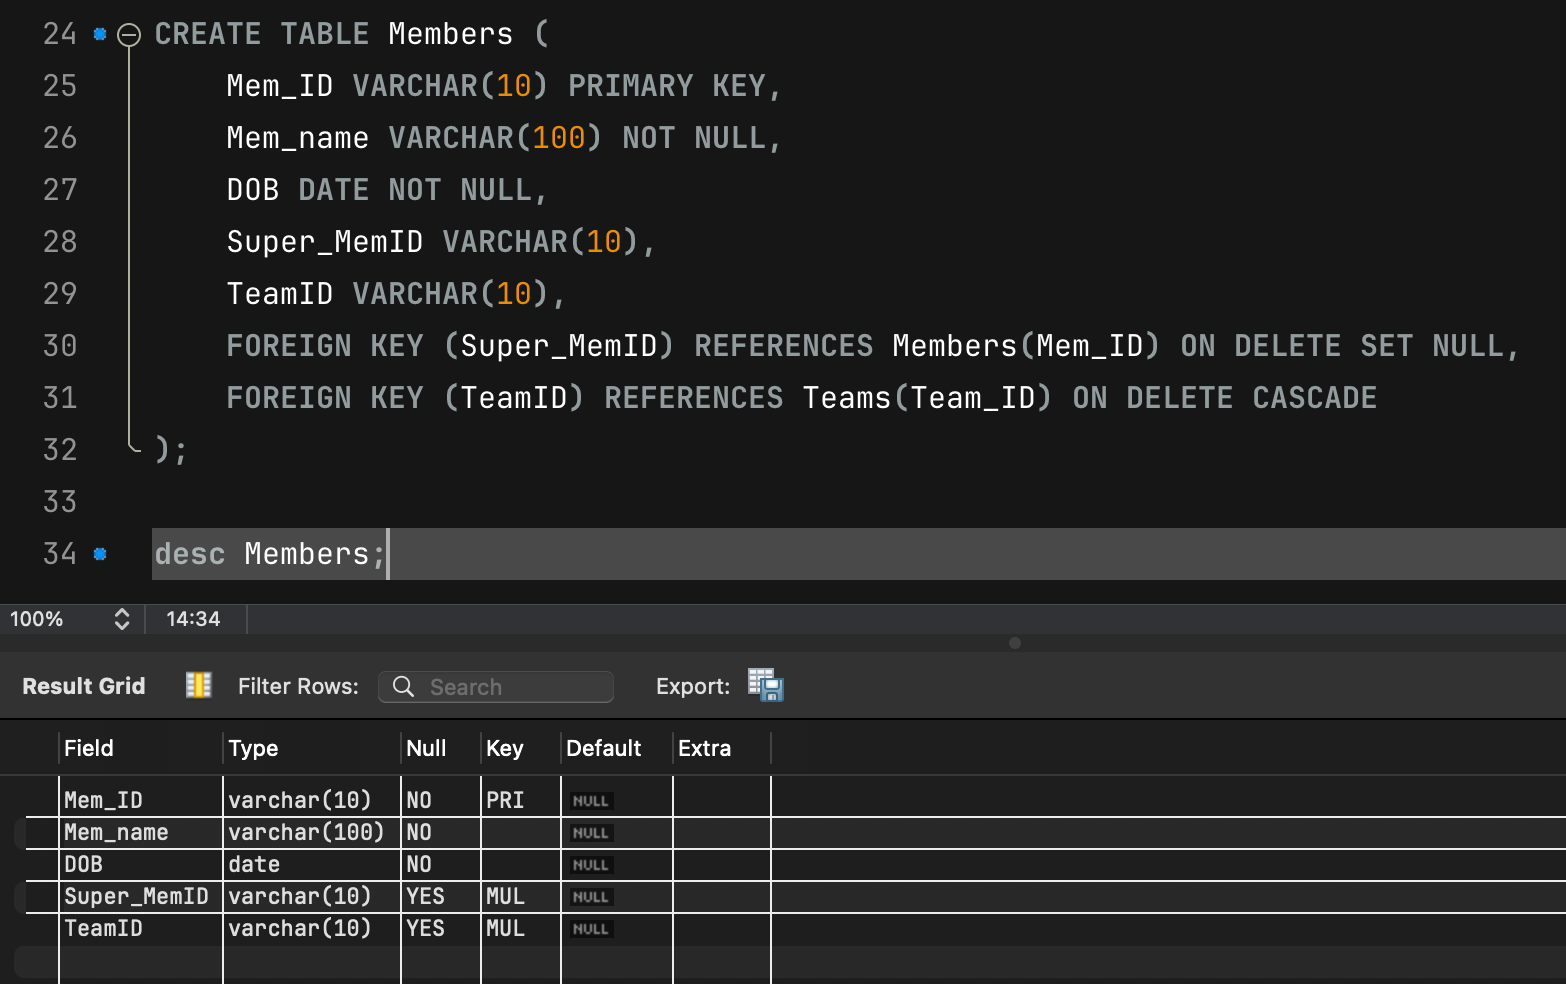
\includegraphics[width=0.7\linewidth]{images/task 1/4.png}
\end{figure}

\begin{figure}[H]
    \centering
    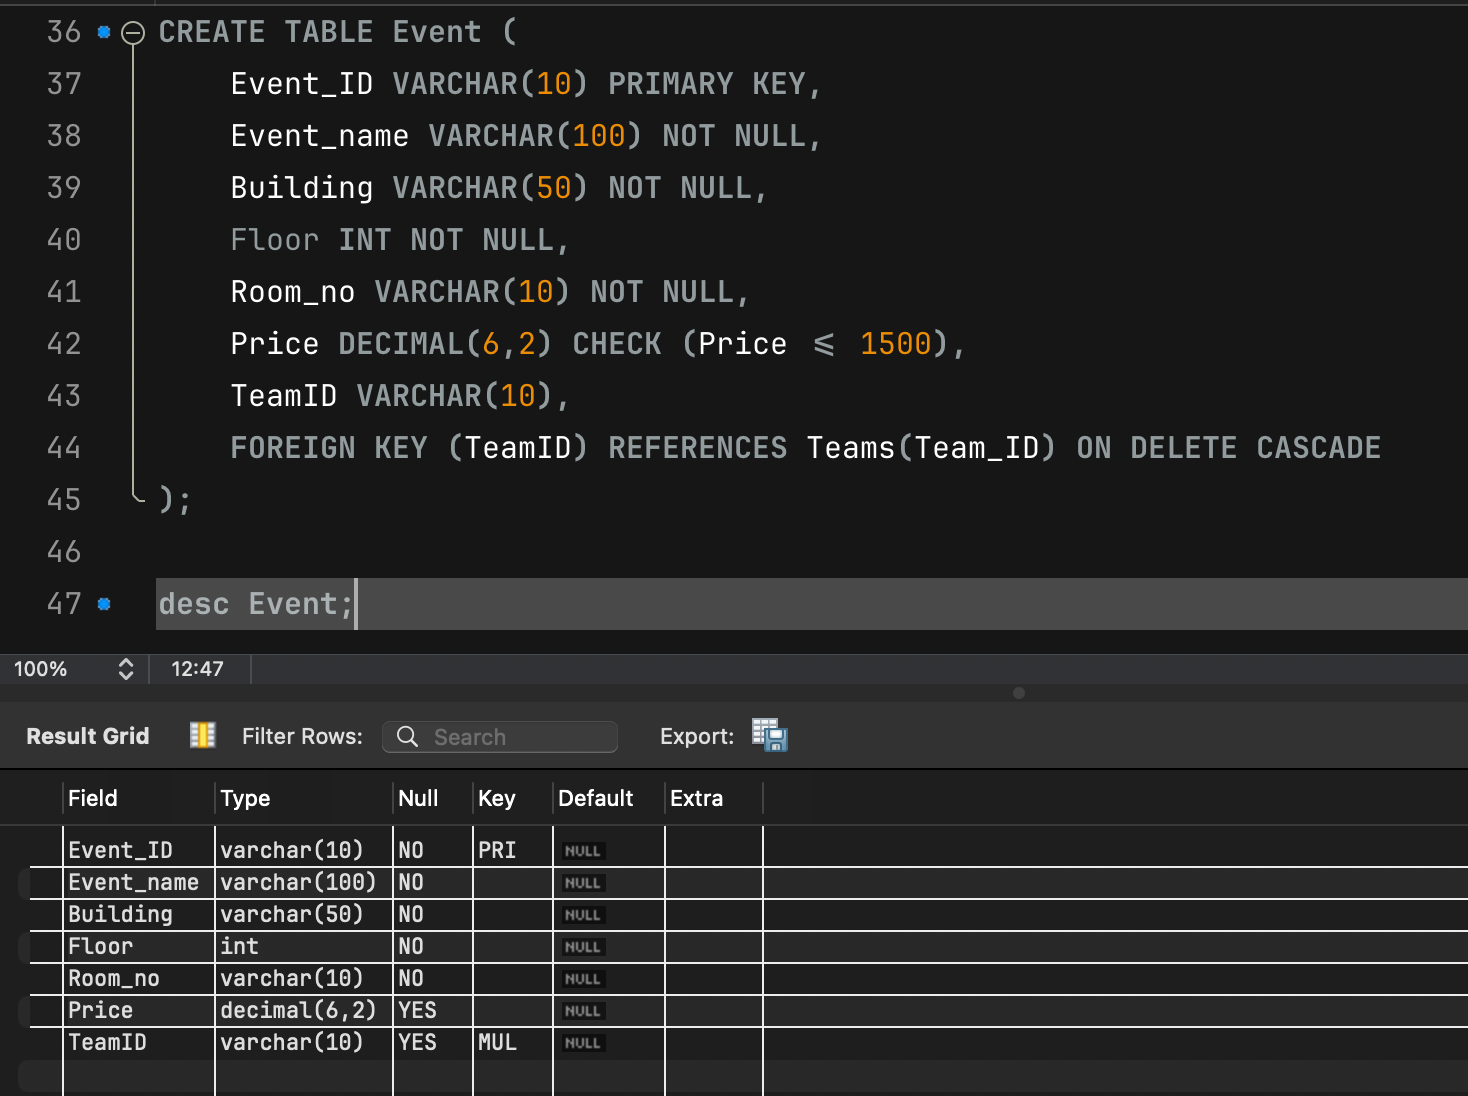
\includegraphics[width=0.7\linewidth]{images/task 1/5.png}
\end{figure}

\begin{figure}[H]
    \centering
    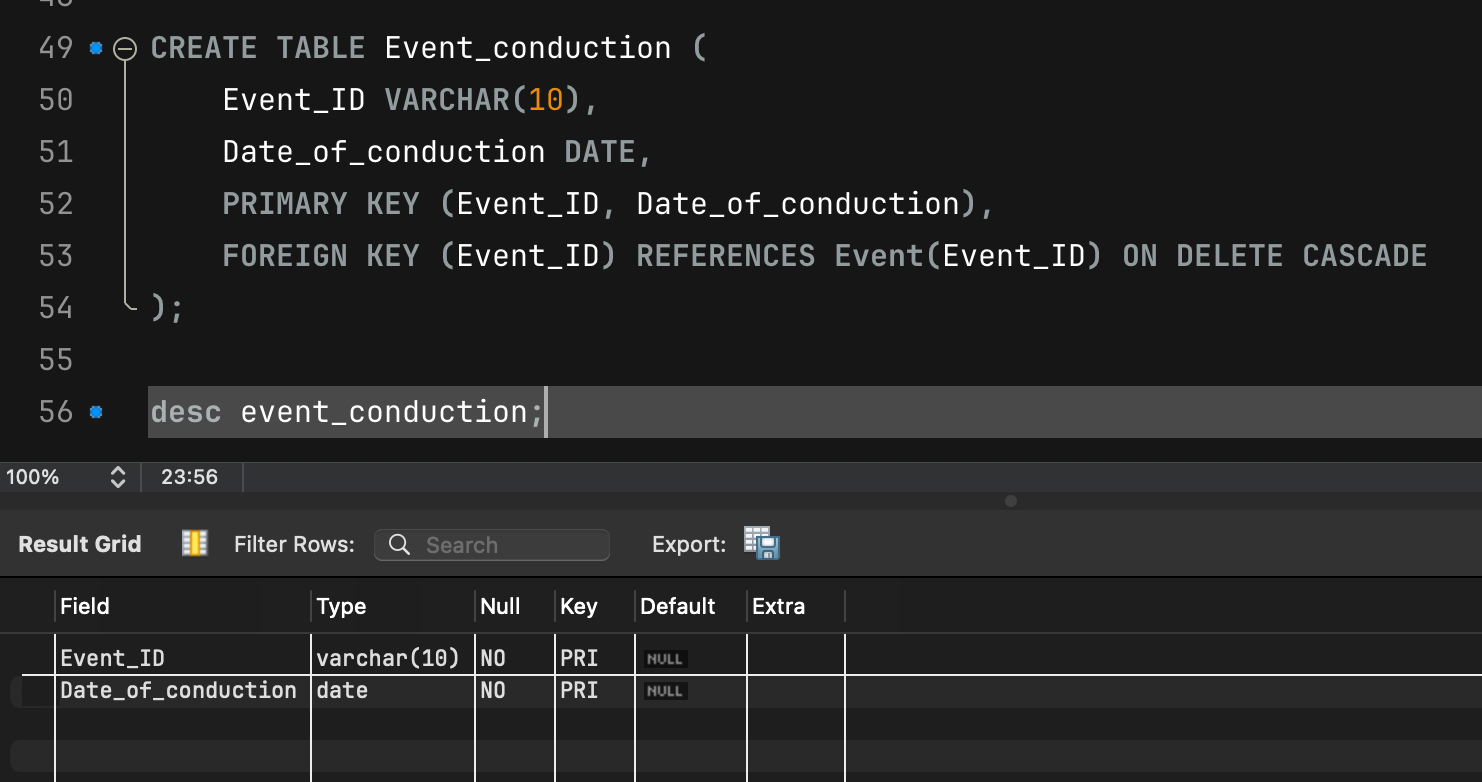
\includegraphics[width=0.7\linewidth]{images/task 1/6.png}
\end{figure}

\begin{figure}[H]
    \centering
    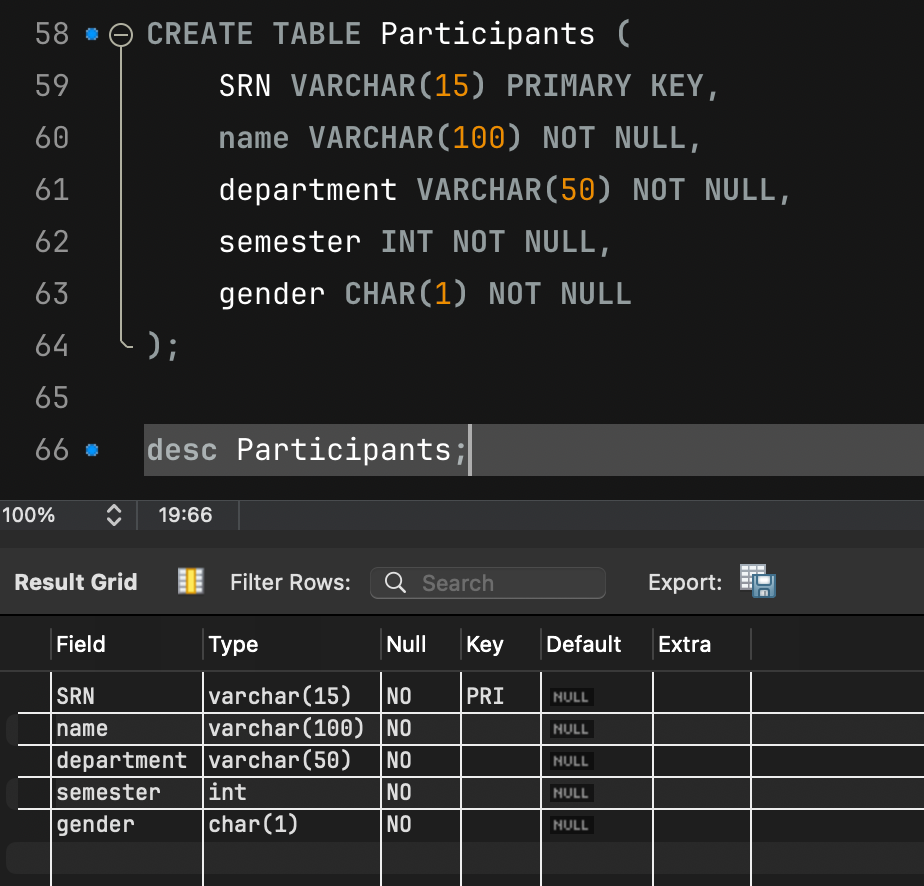
\includegraphics[width=0.7\linewidth]{images/task 1/7.png}
\end{figure}

\begin{figure}[H]
    \centering
    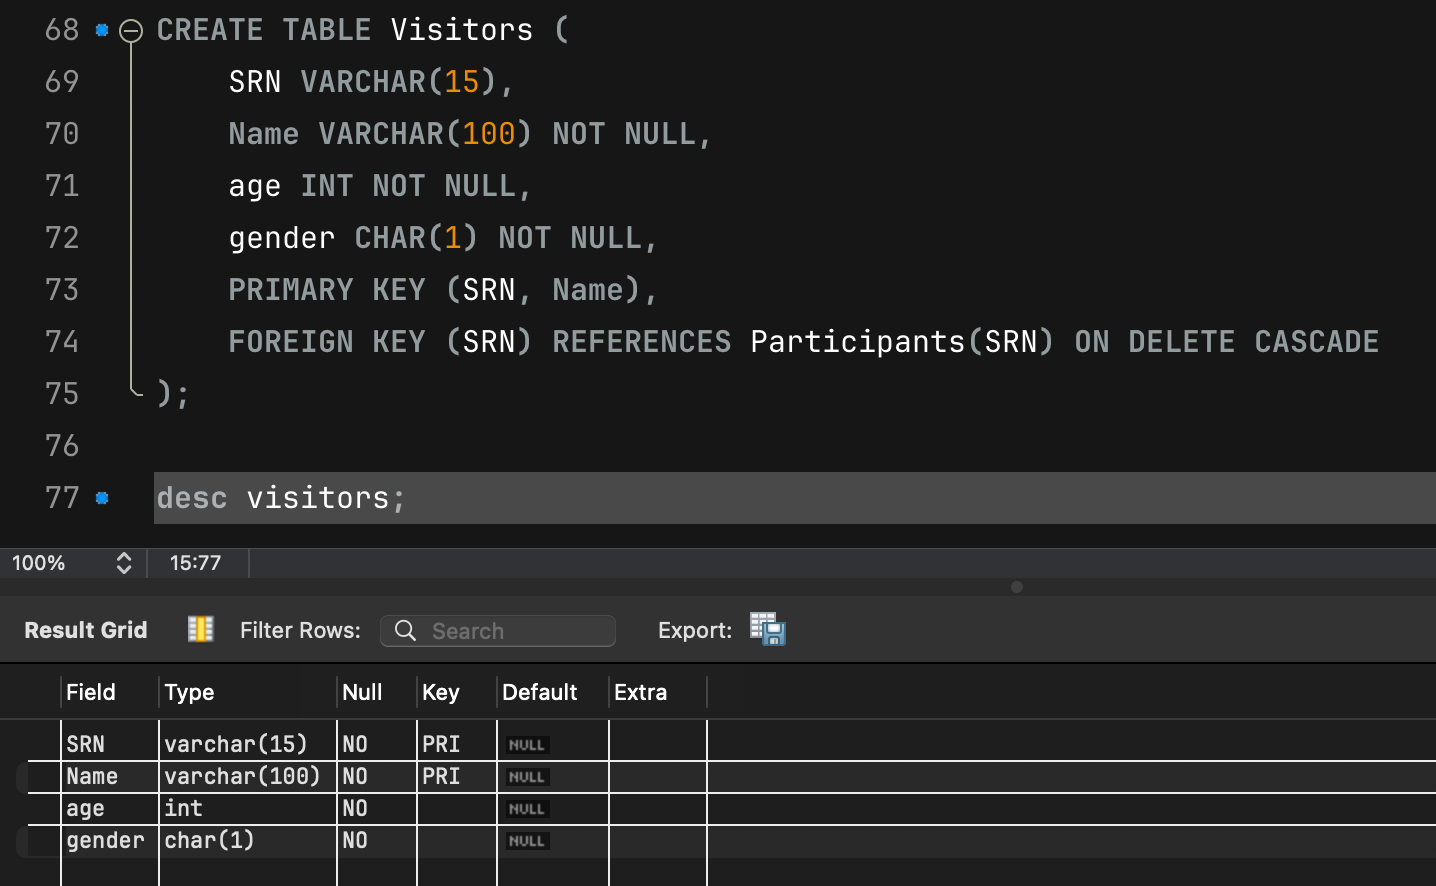
\includegraphics[width=0.7\linewidth]{images/task 1/8.png}
\end{figure}

\begin{figure}[H]
    \centering
    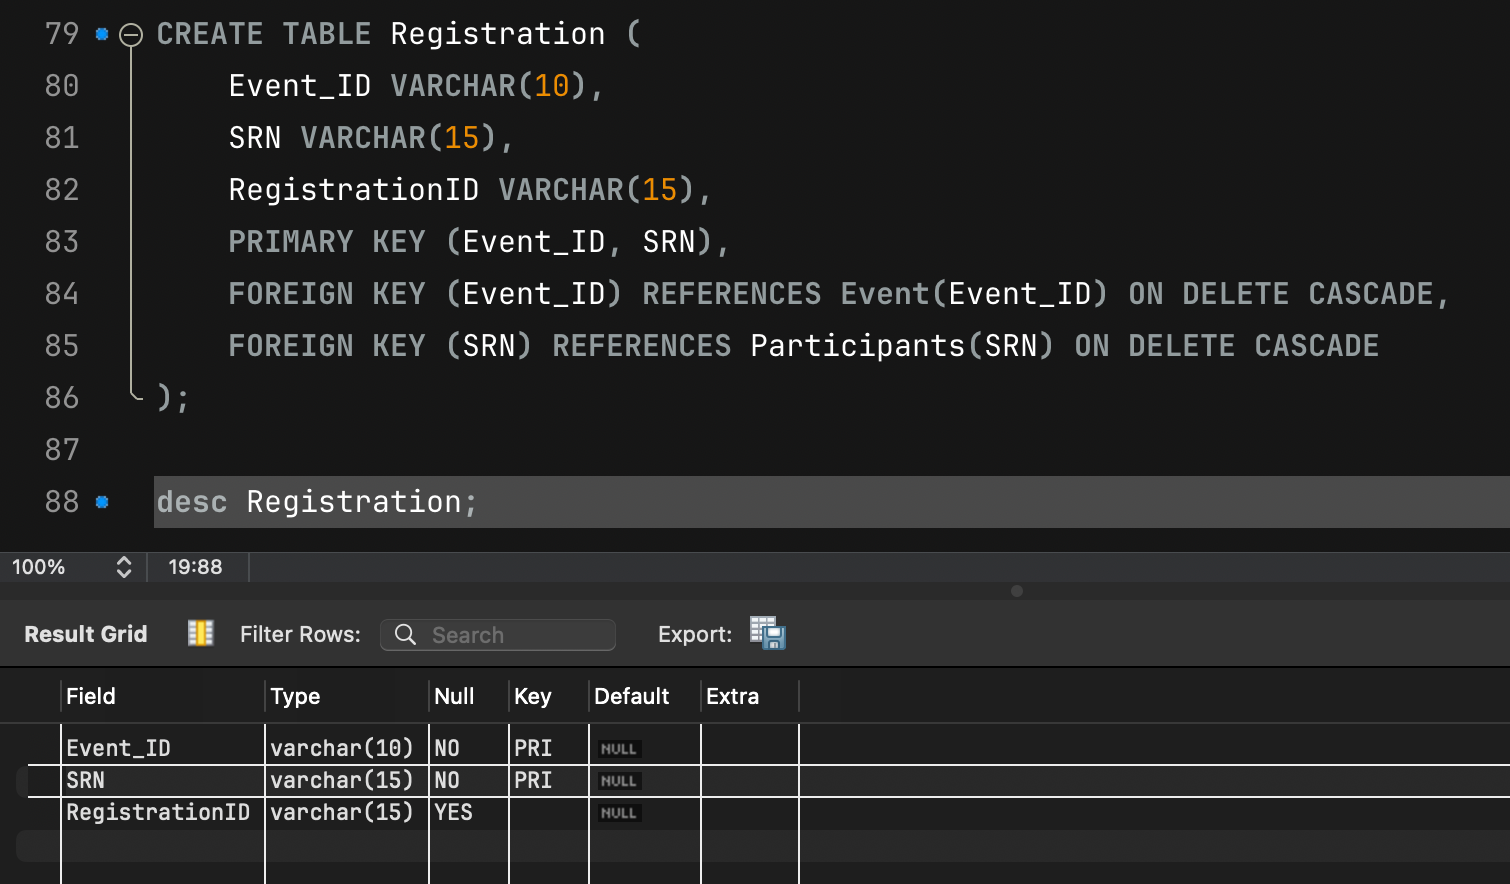
\includegraphics[width=0.7\linewidth]{images/task 1/9.png}
\end{figure}

\begin{figure}[H]
    \centering
    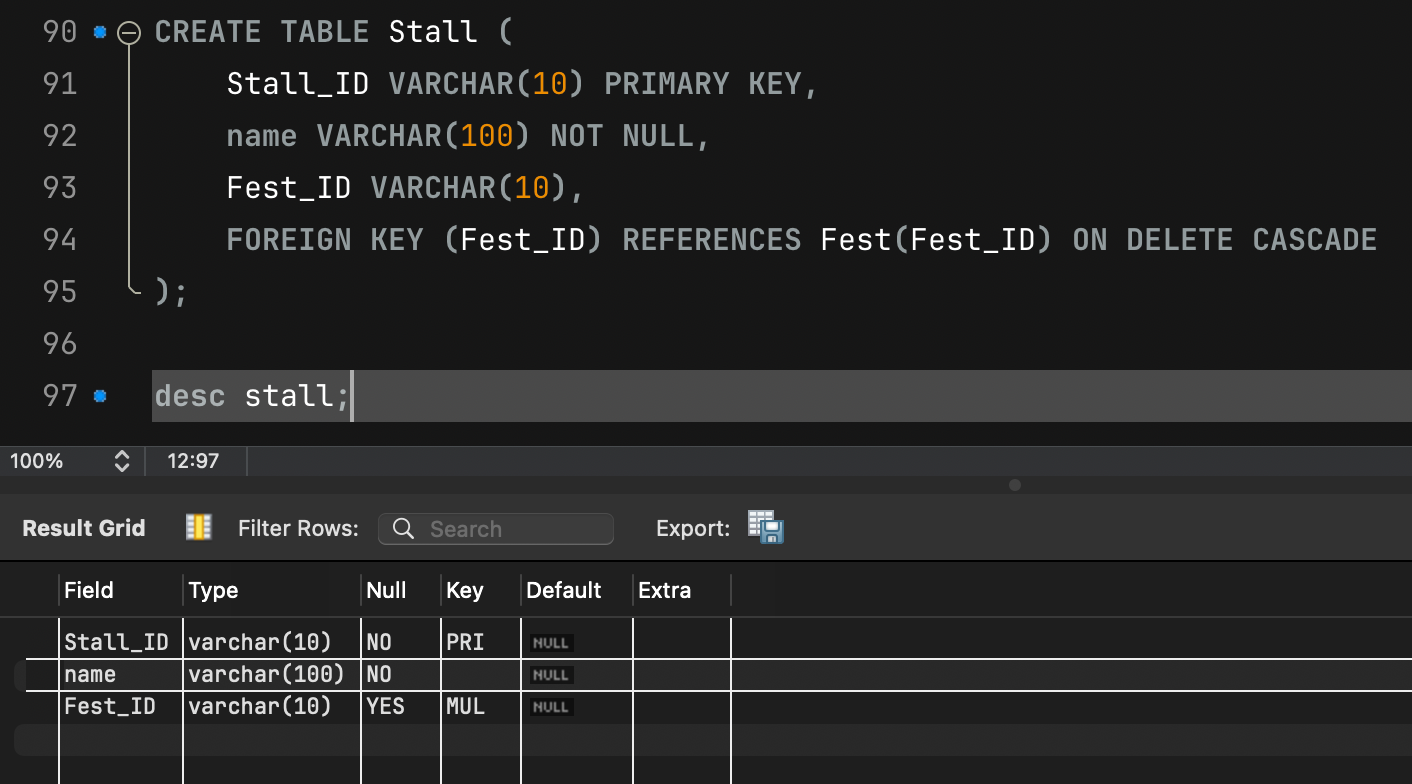
\includegraphics[width=0.7\linewidth]{images/task 1/10.png}
\end{figure}

\begin{figure}[H]
    \centering
    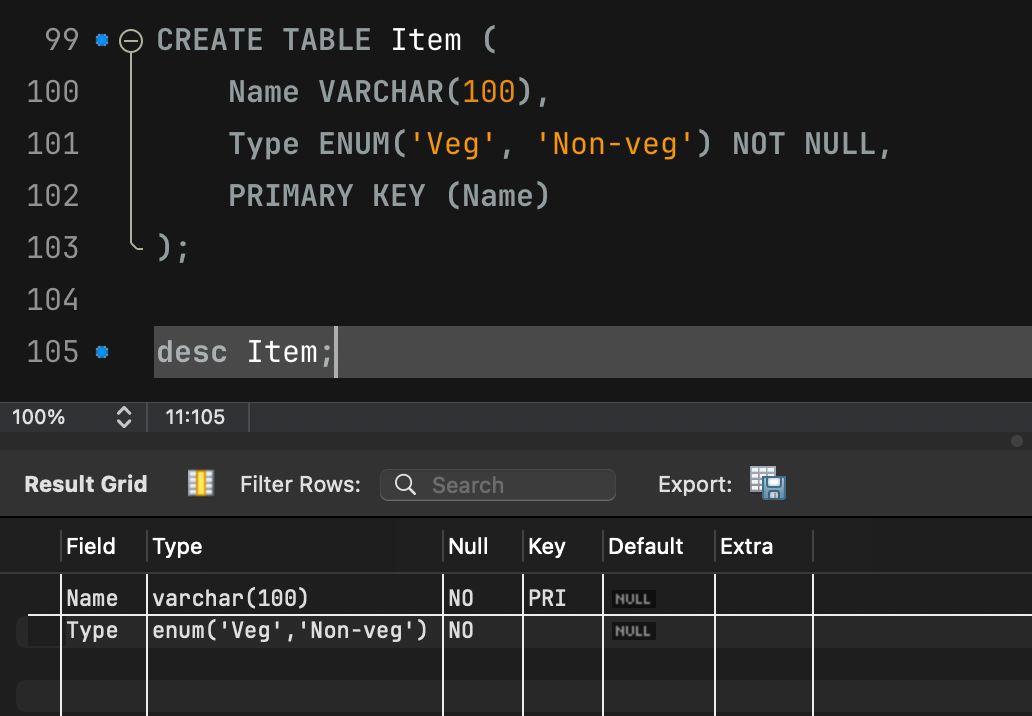
\includegraphics[width=0.7\linewidth]{images/task 1/11.png}
\end{figure}

\begin{figure}[H]
    \centering
    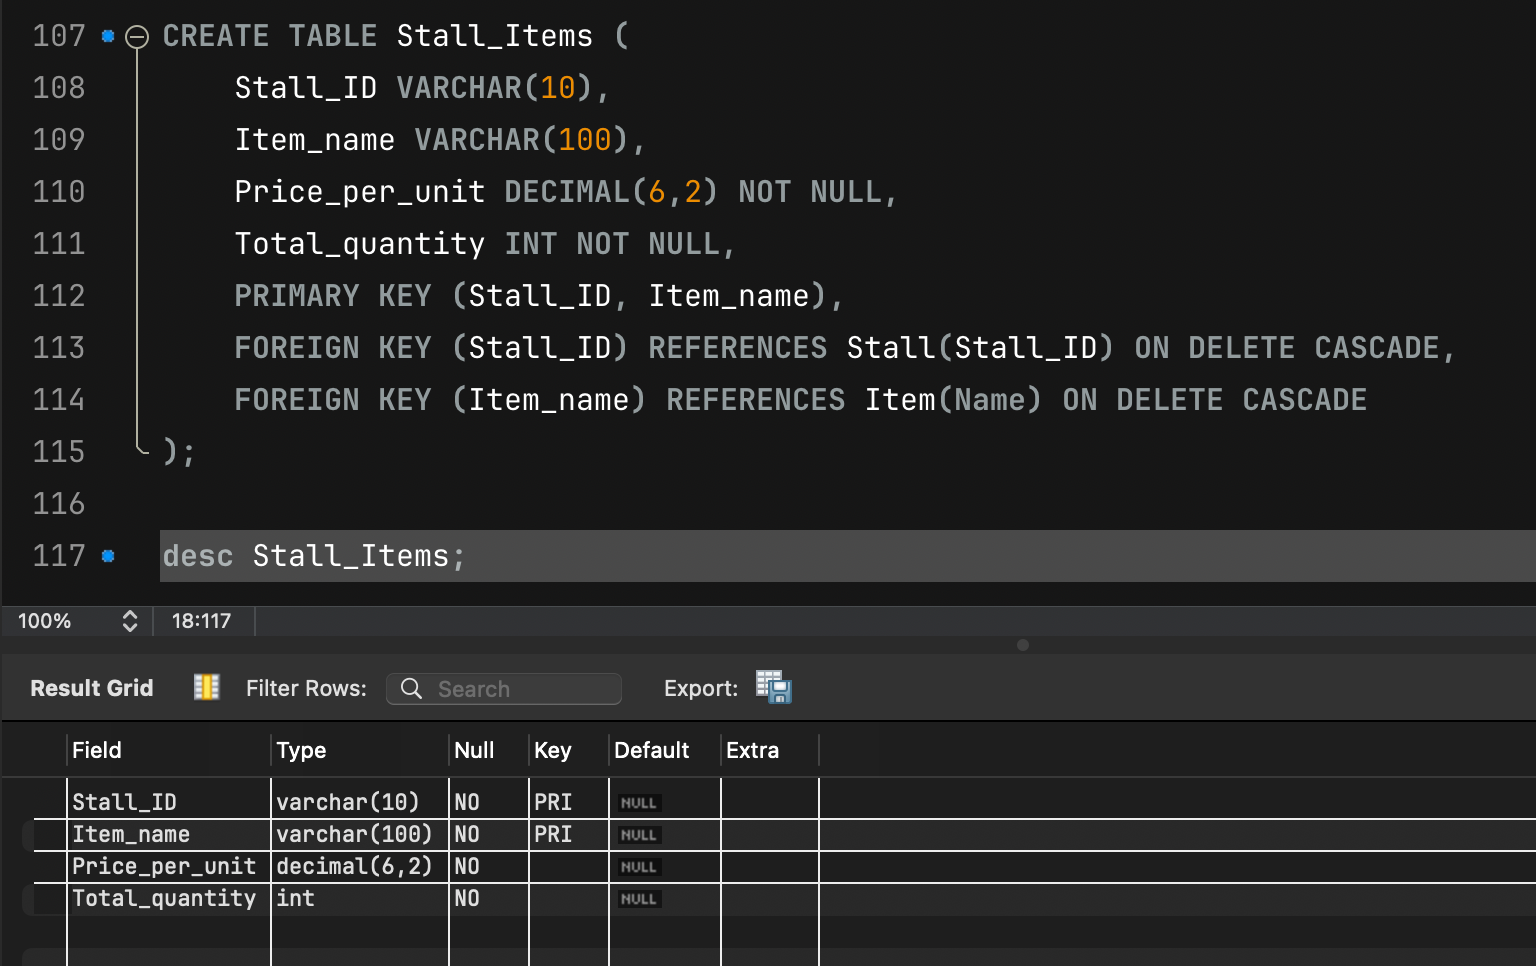
\includegraphics[width=0.7\linewidth]{images/task 1/12.png}
\end{figure}

\begin{figure}[H]
    \centering
    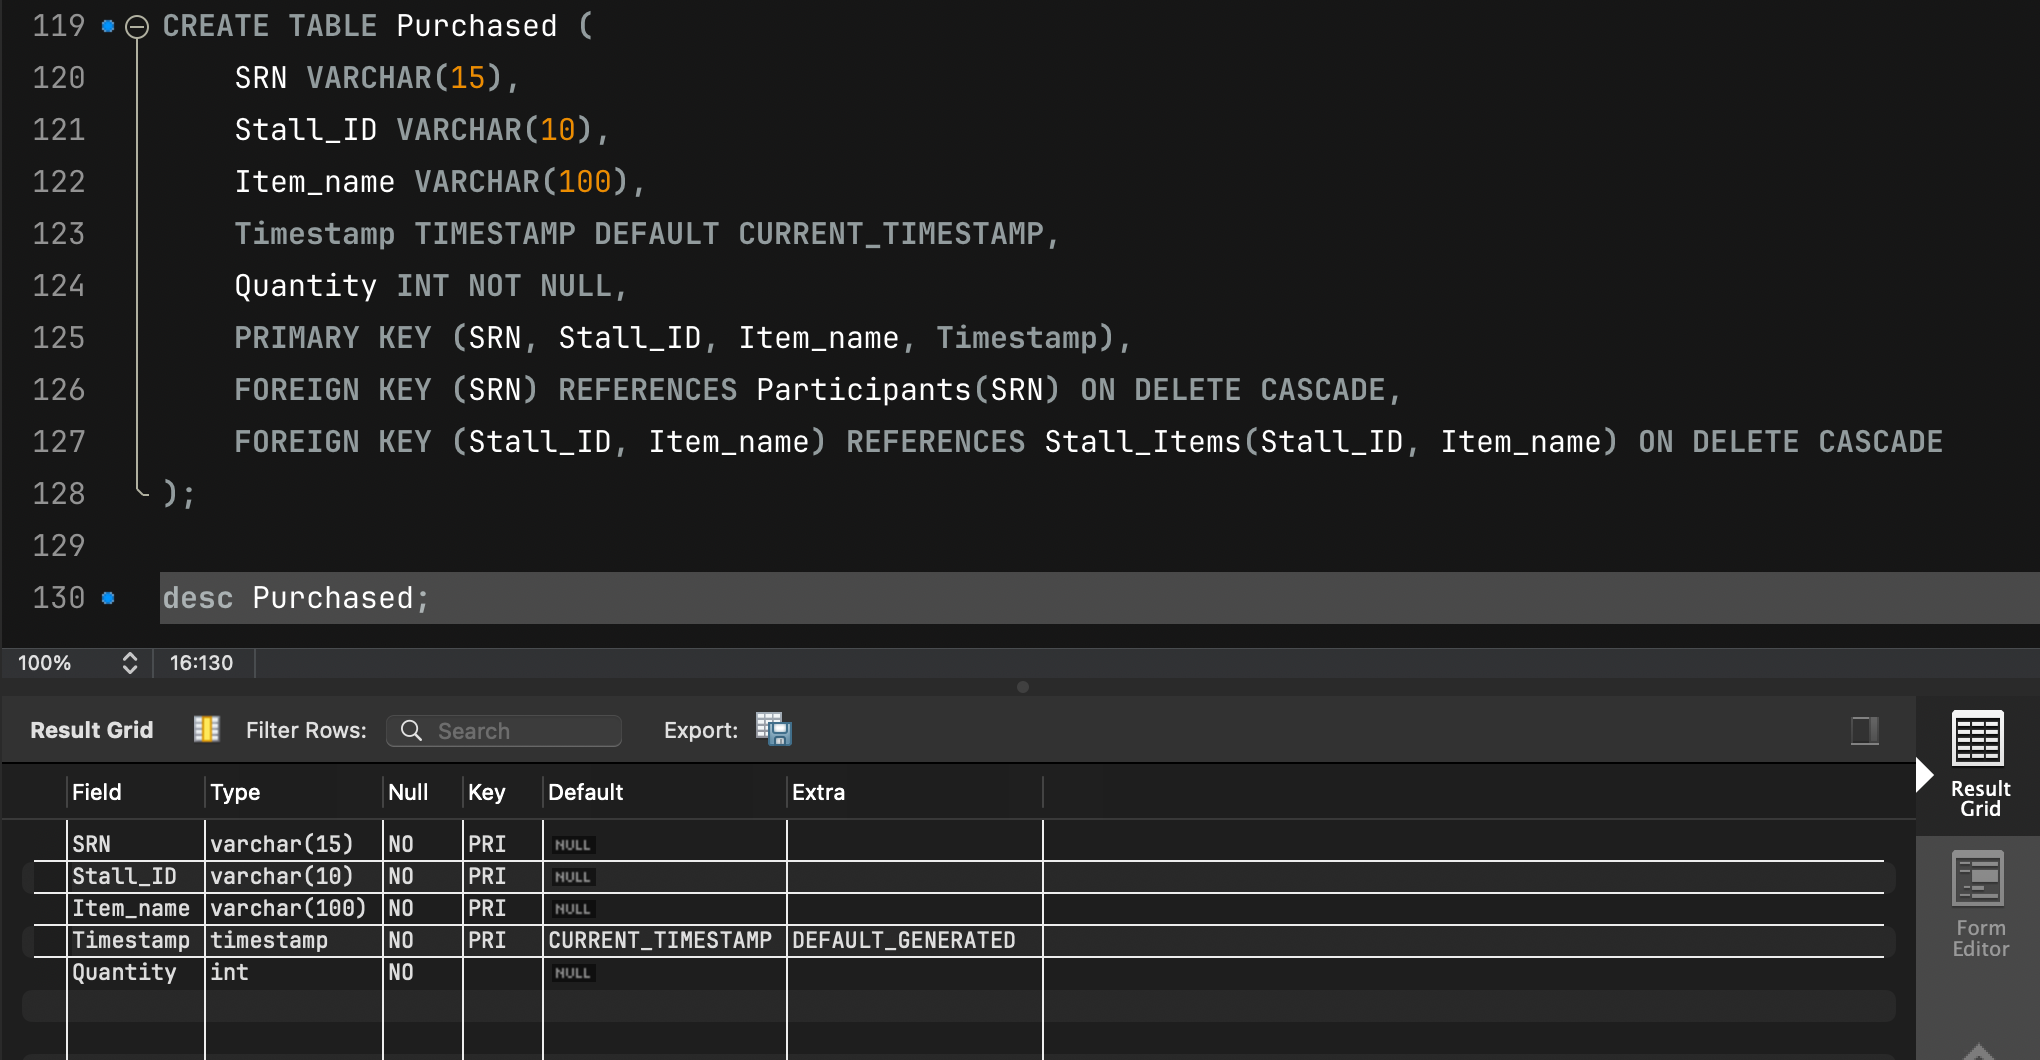
\includegraphics[width=0.7\linewidth]{images/task 1/13.png}
\end{figure}

\begin{figure}[H]
    \centering
    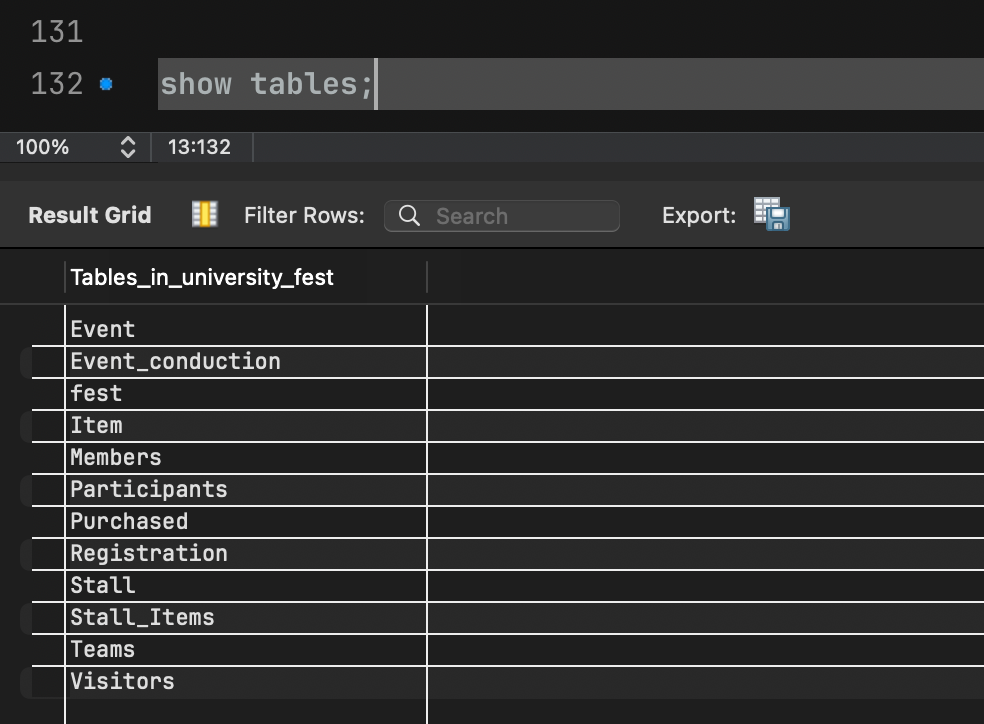
\includegraphics[width=0.7\linewidth]{images/task 1/14.png}
\end{figure}

\newpage

\section{Task 2}

\begin{figure}[H]
    \centering
    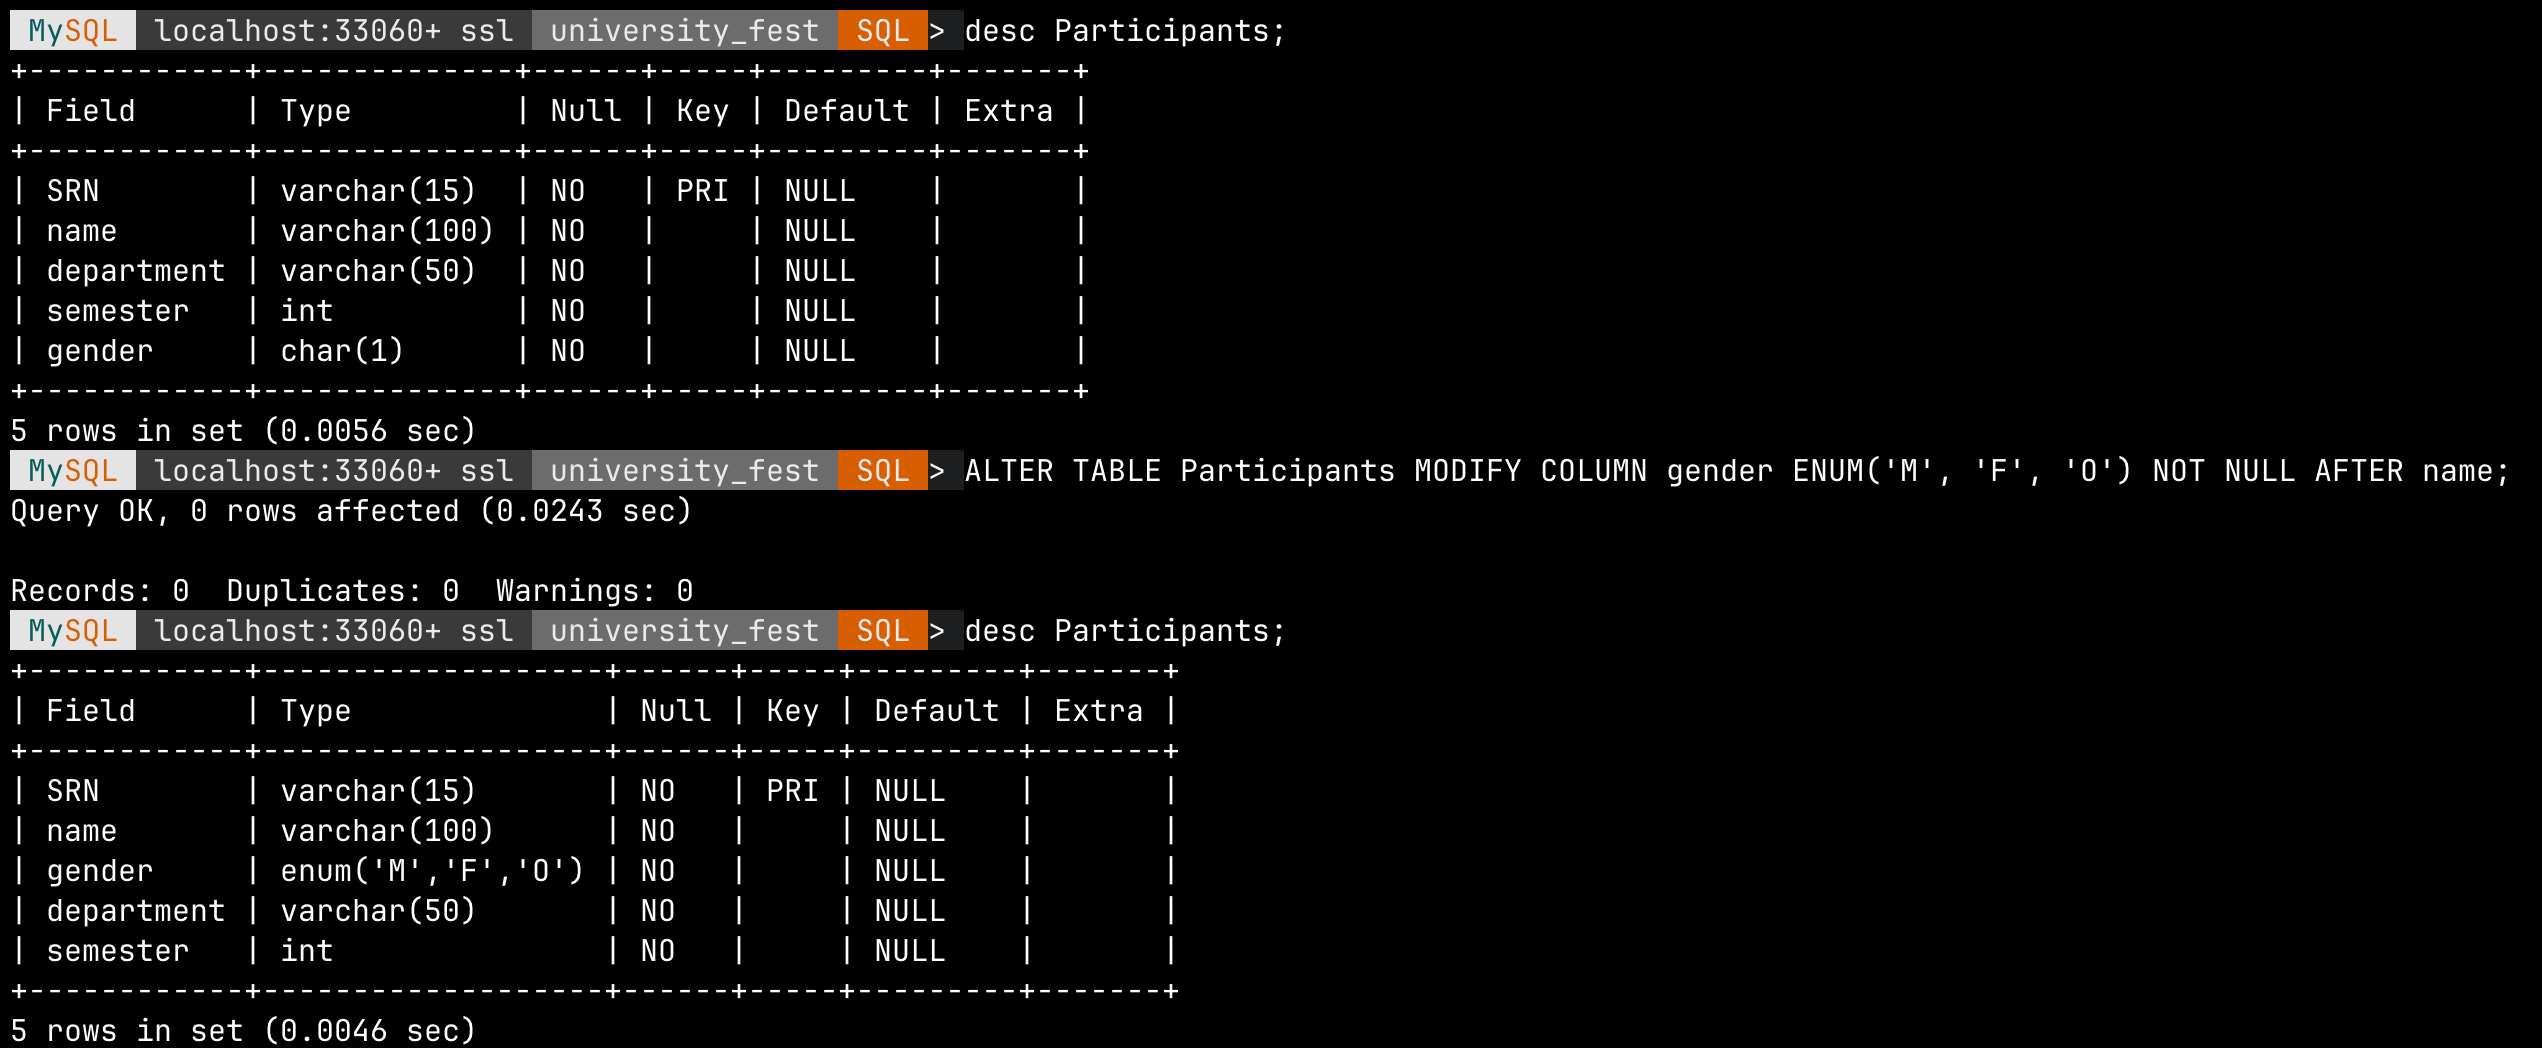
\includegraphics[width=0.7\linewidth]{images/task 2/1.png}
\end{figure}

\begin{figure}[H]
    \centering
    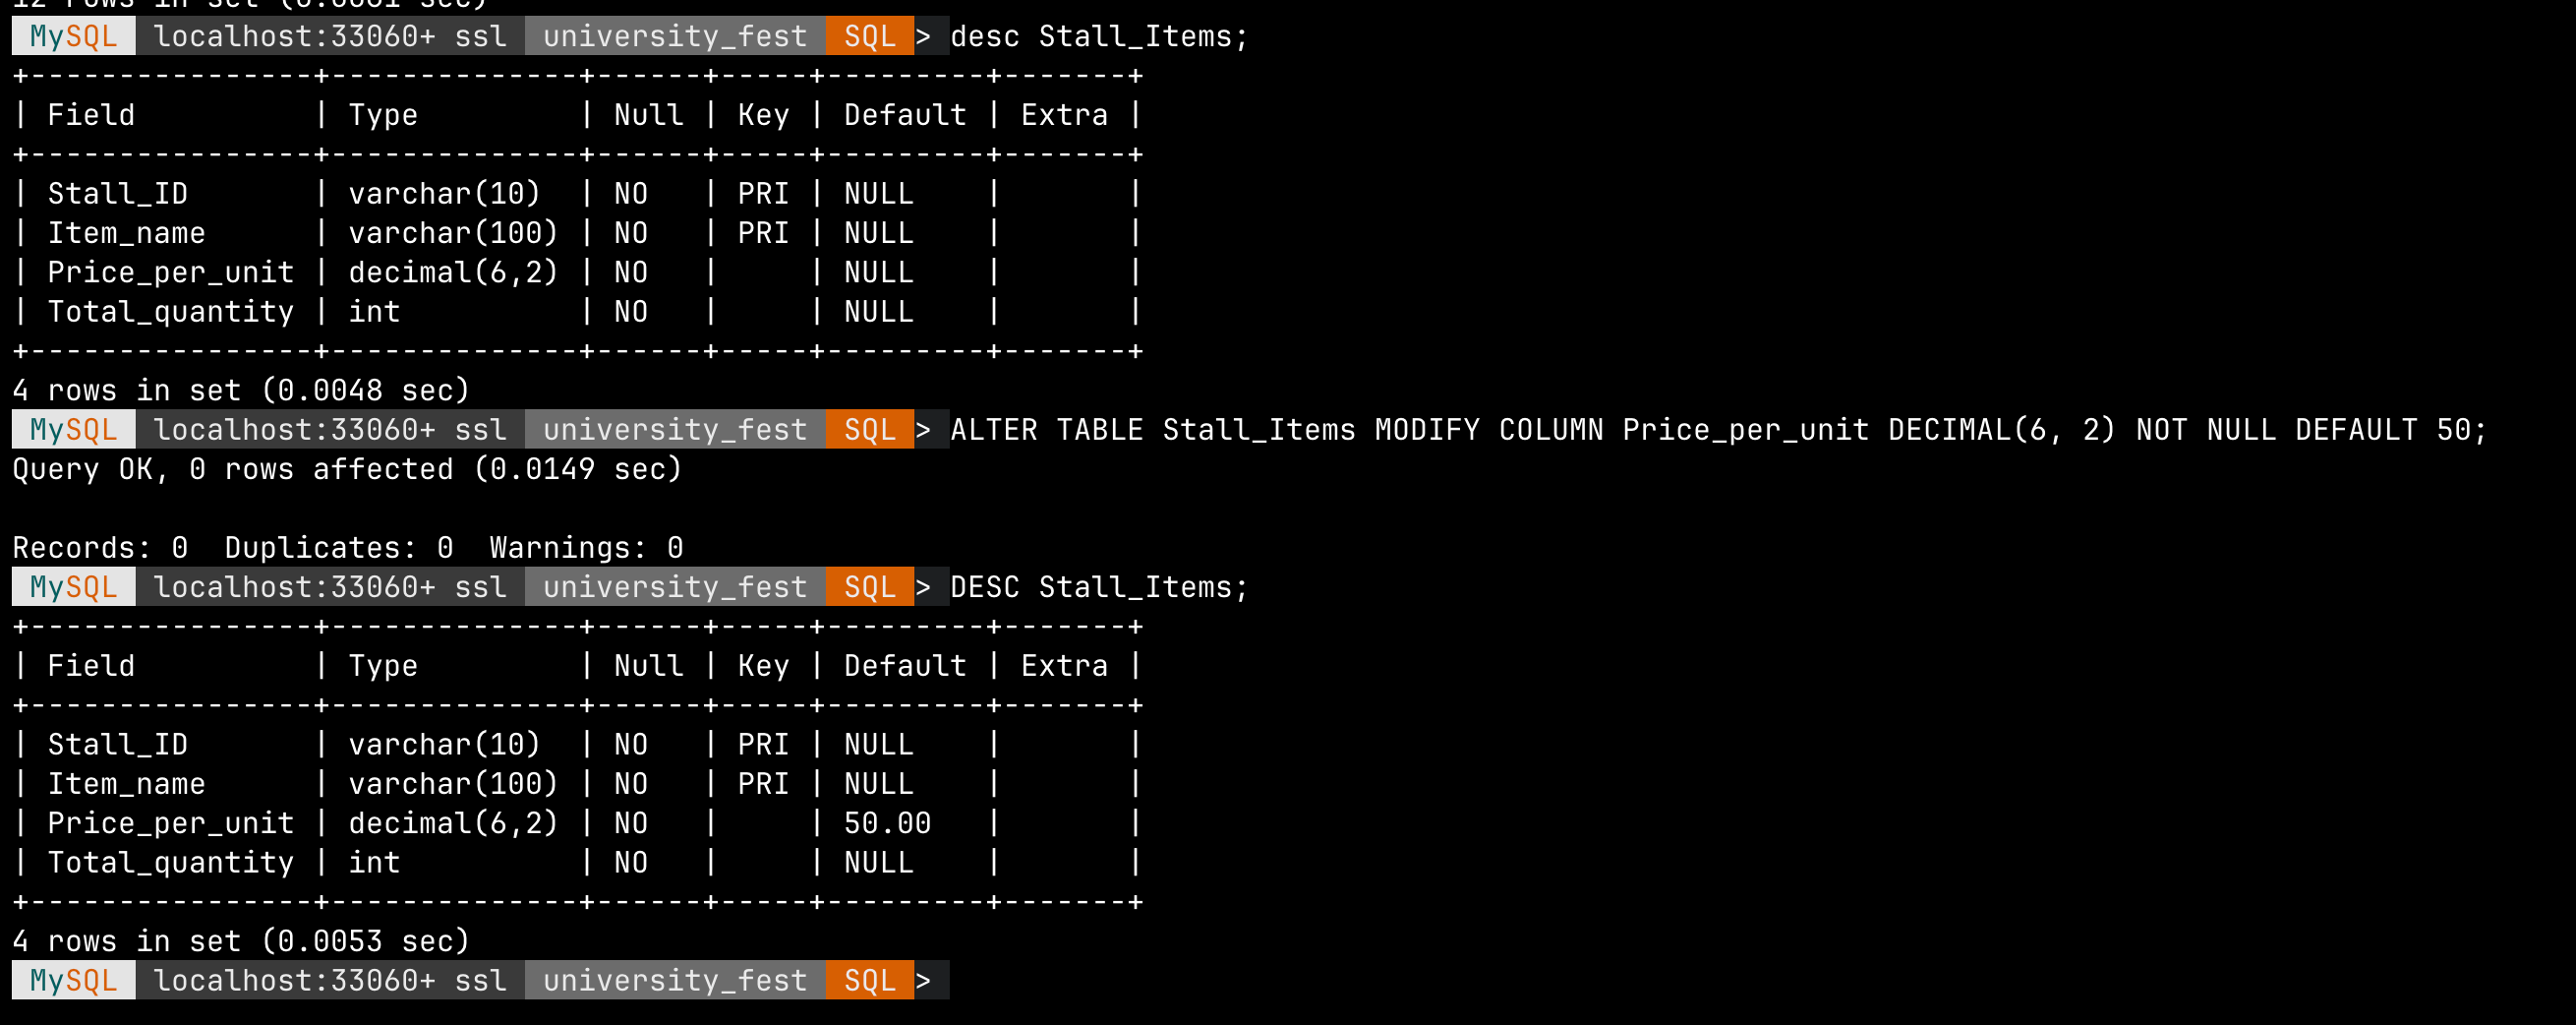
\includegraphics[width=0.7\linewidth]{images/task 2/2.png}
\end{figure}

\begin{figure}[H]
    \centering
    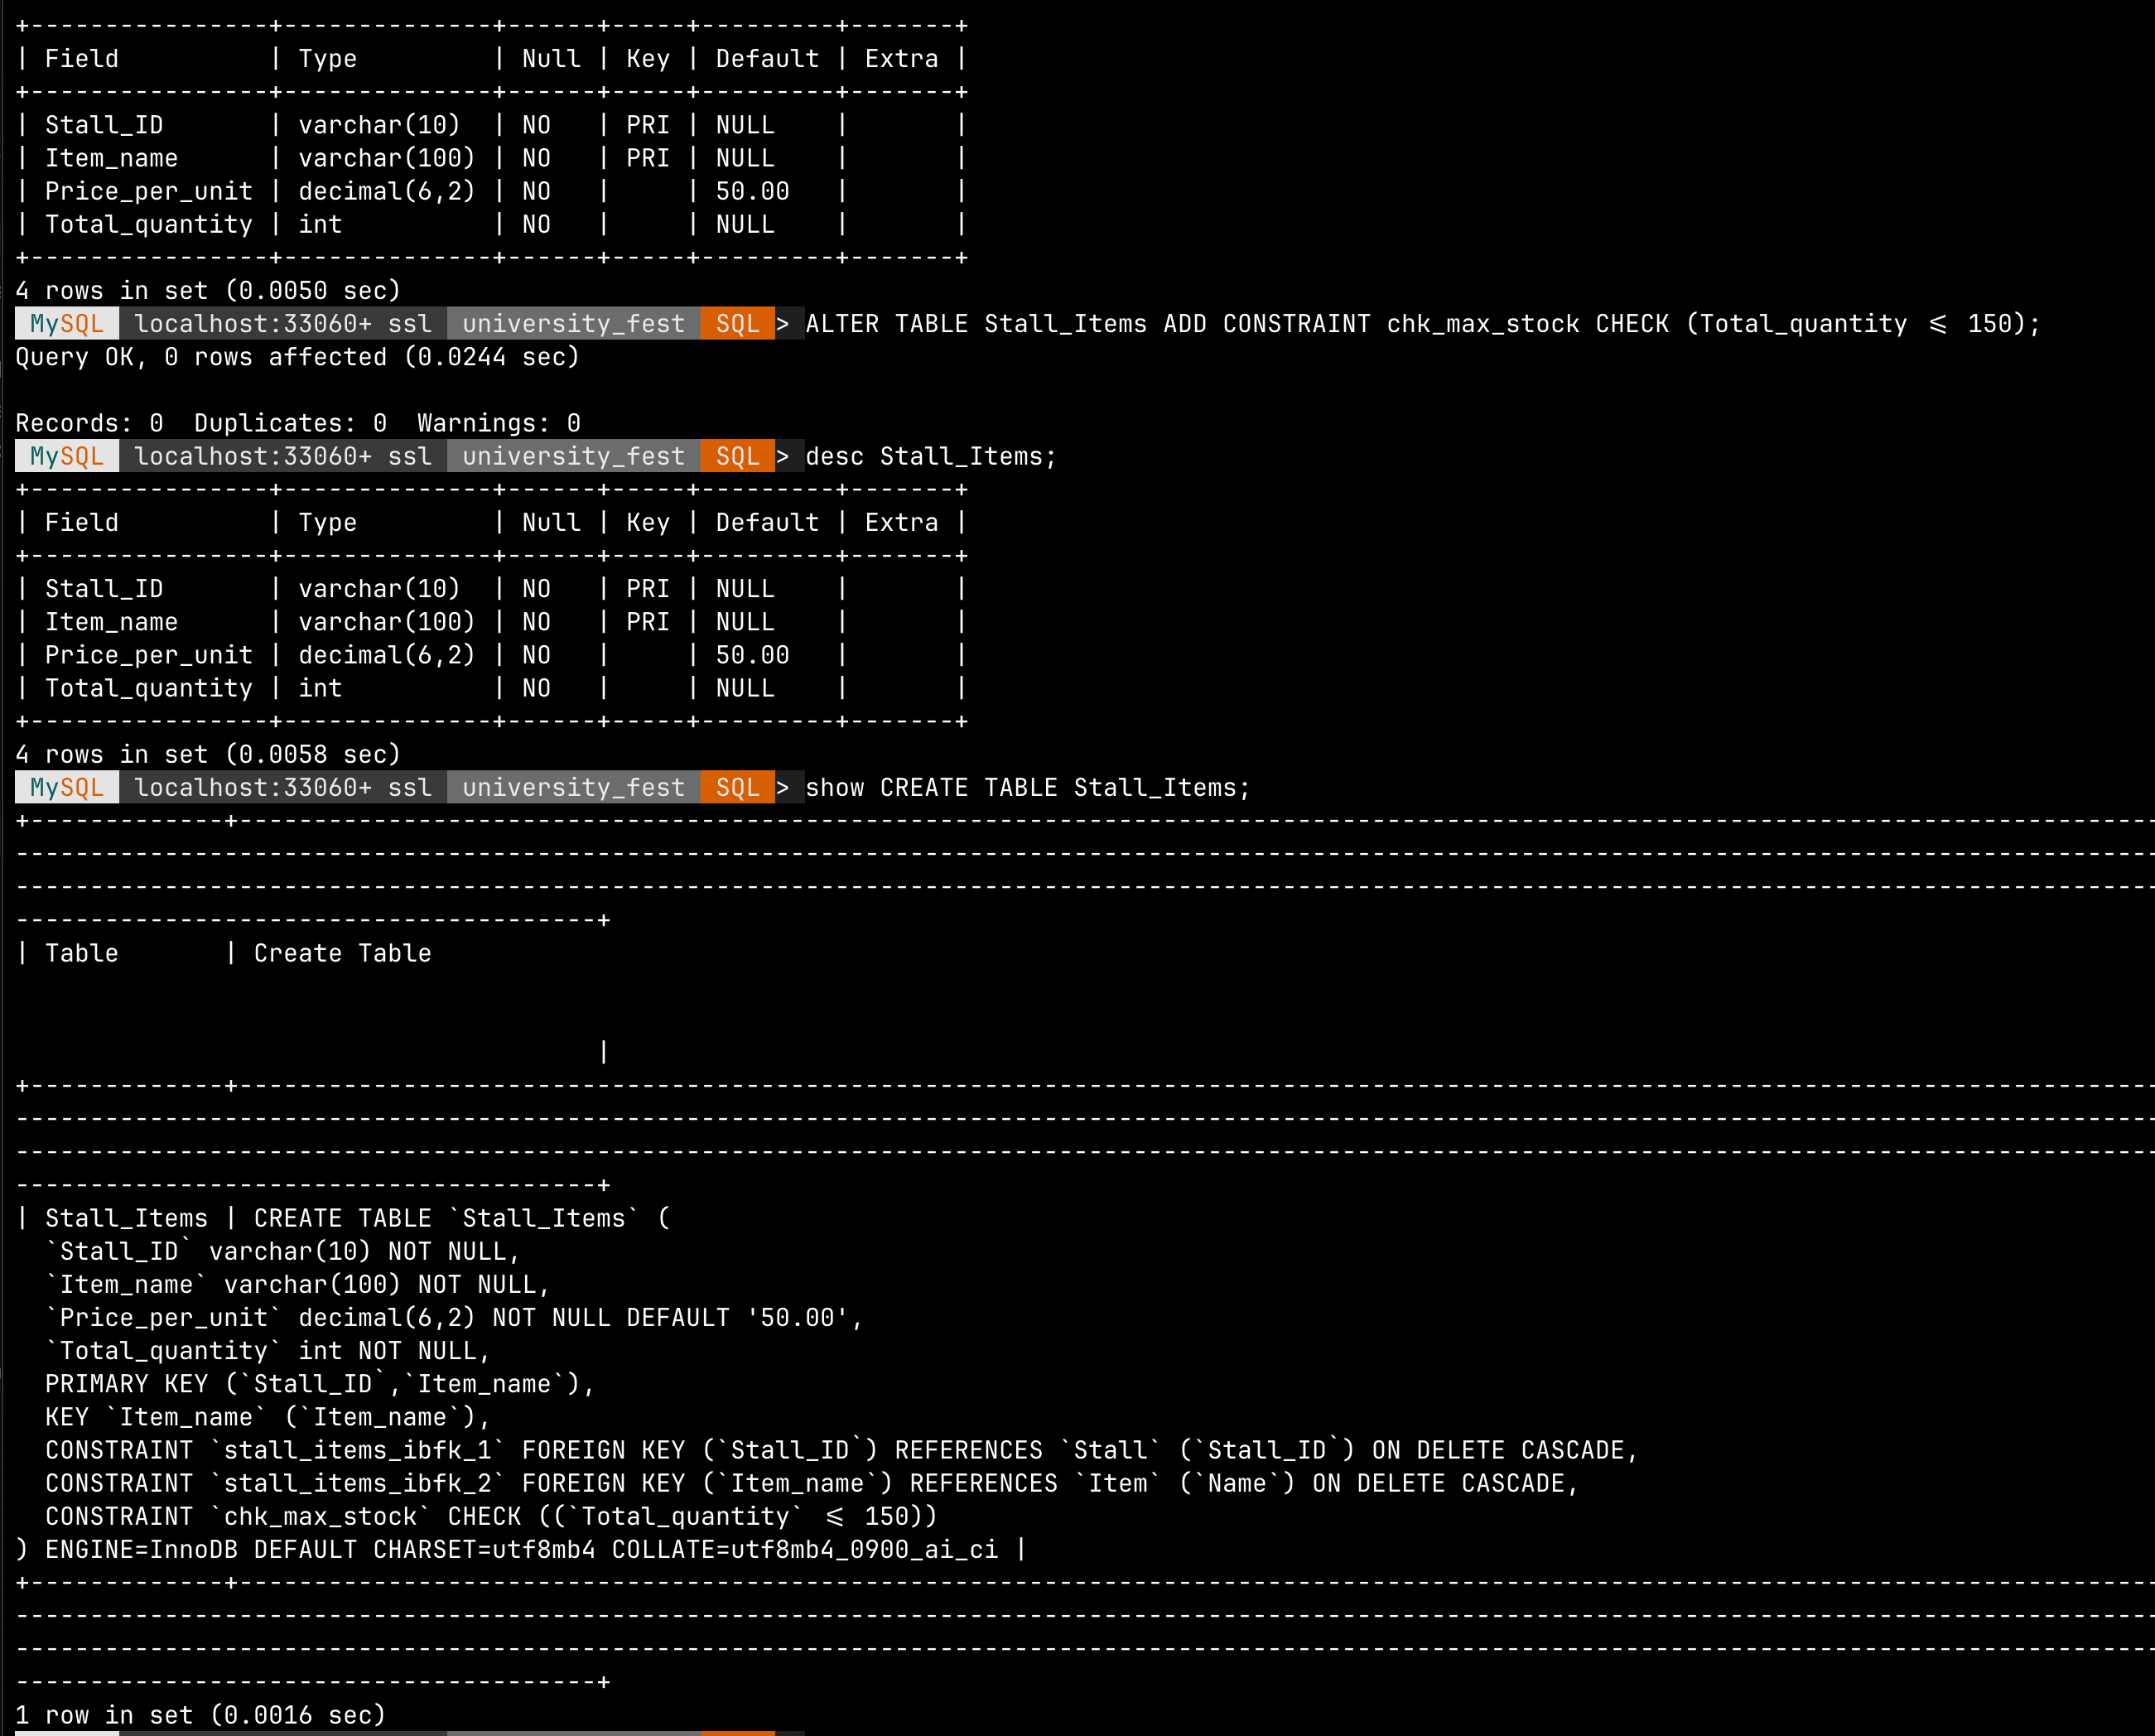
\includegraphics[width=0.7\linewidth]{images/task 2/3.png}
\end{figure}

\begin{figure}[H]
    \centering
    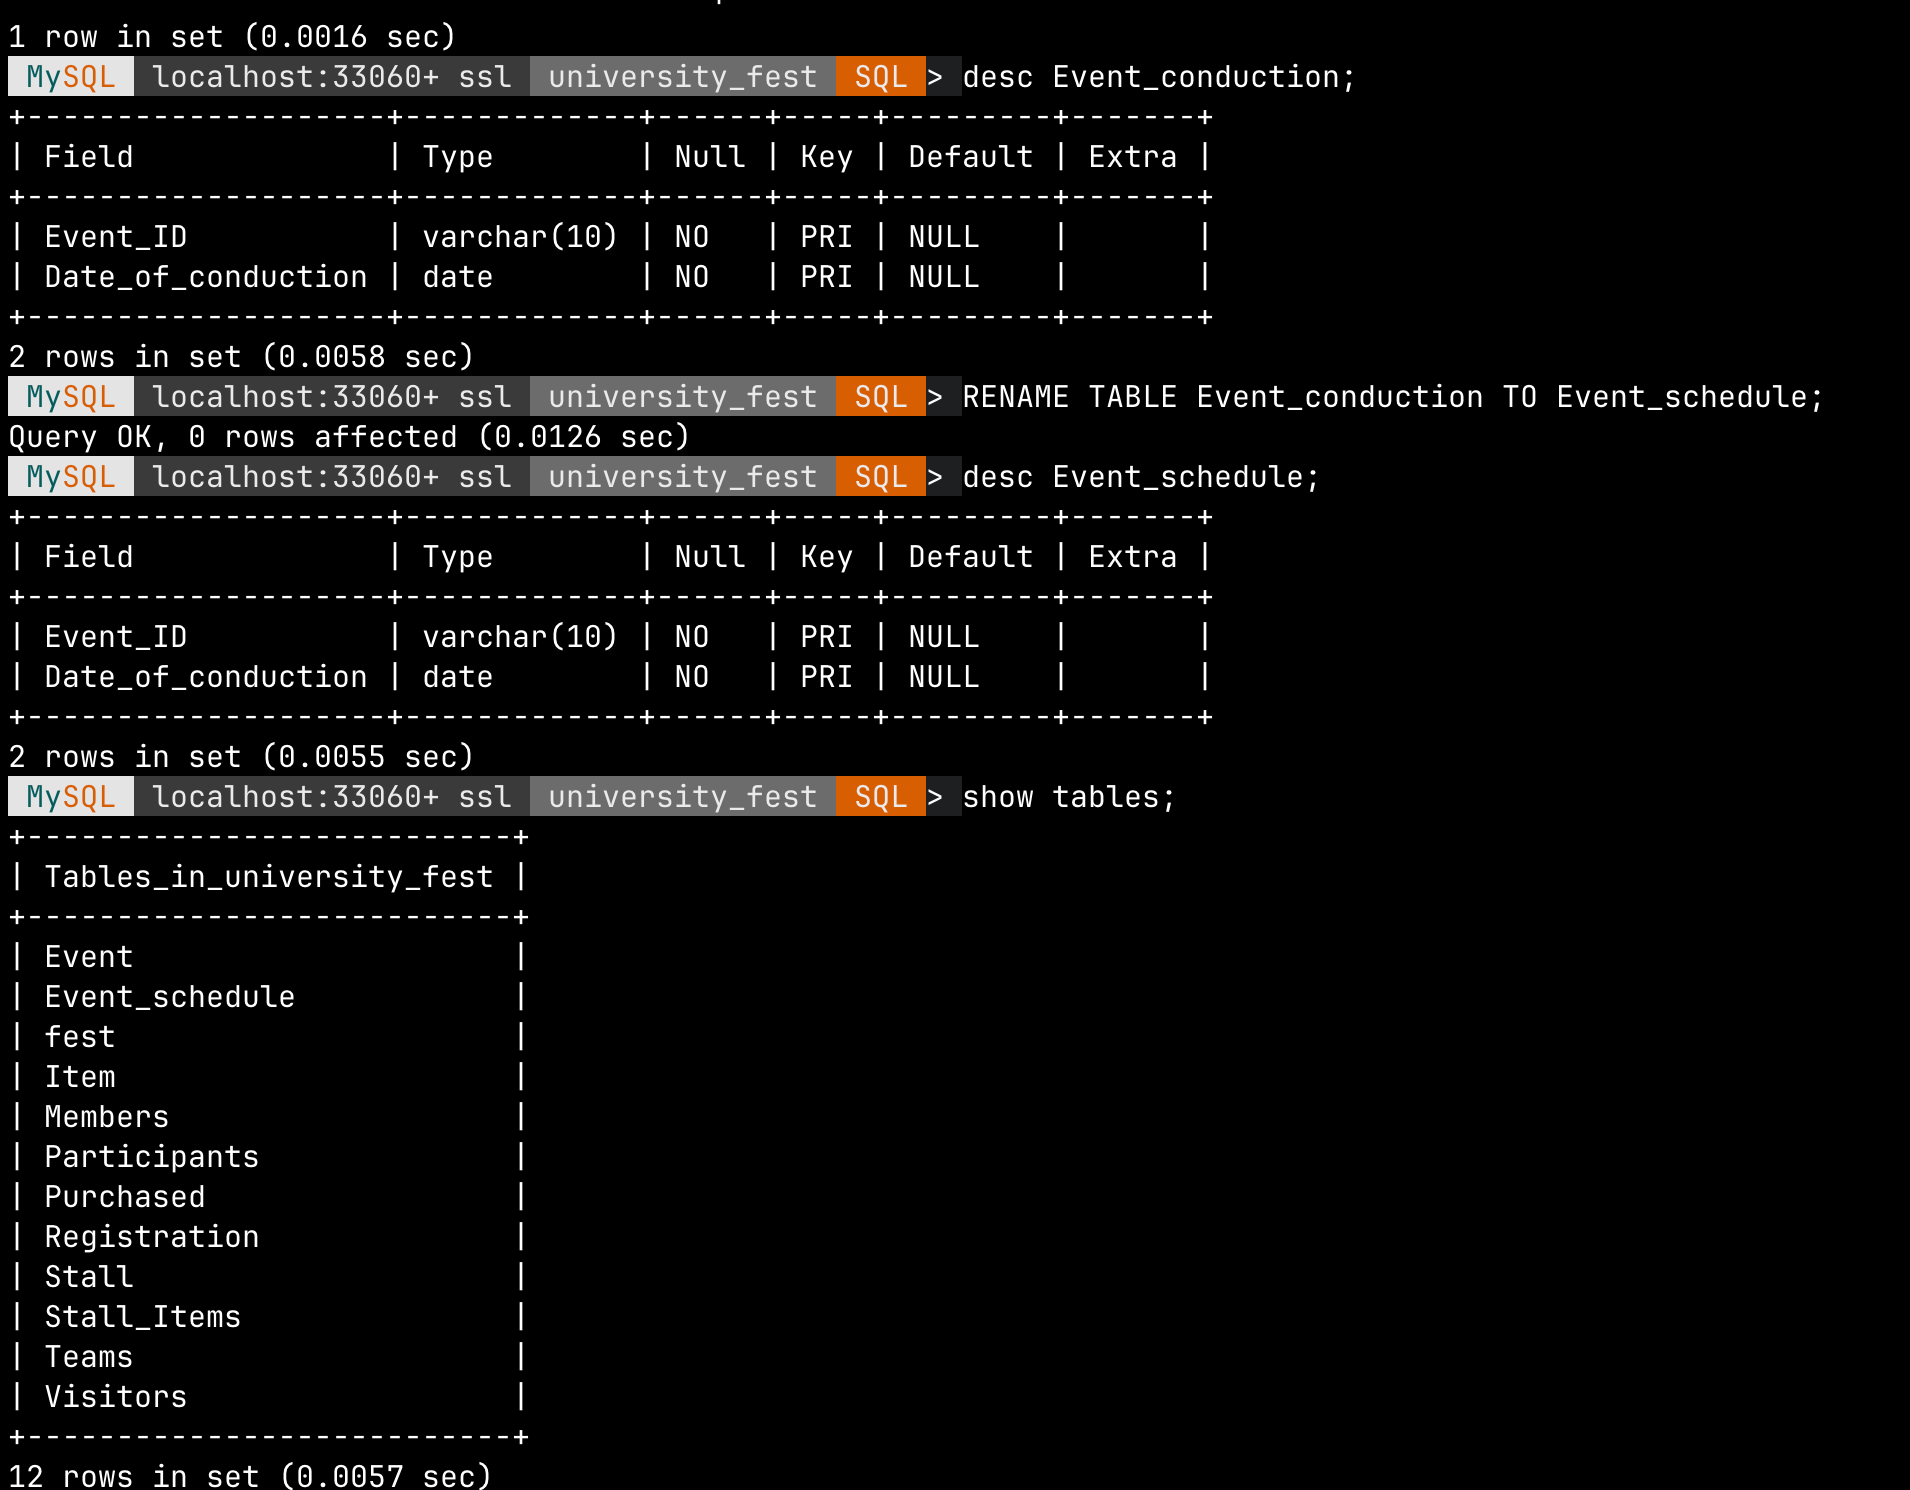
\includegraphics[width=0.7\linewidth]{images/task 2/4.png}
\end{figure}

\begin{figure}[H]
    \centering
    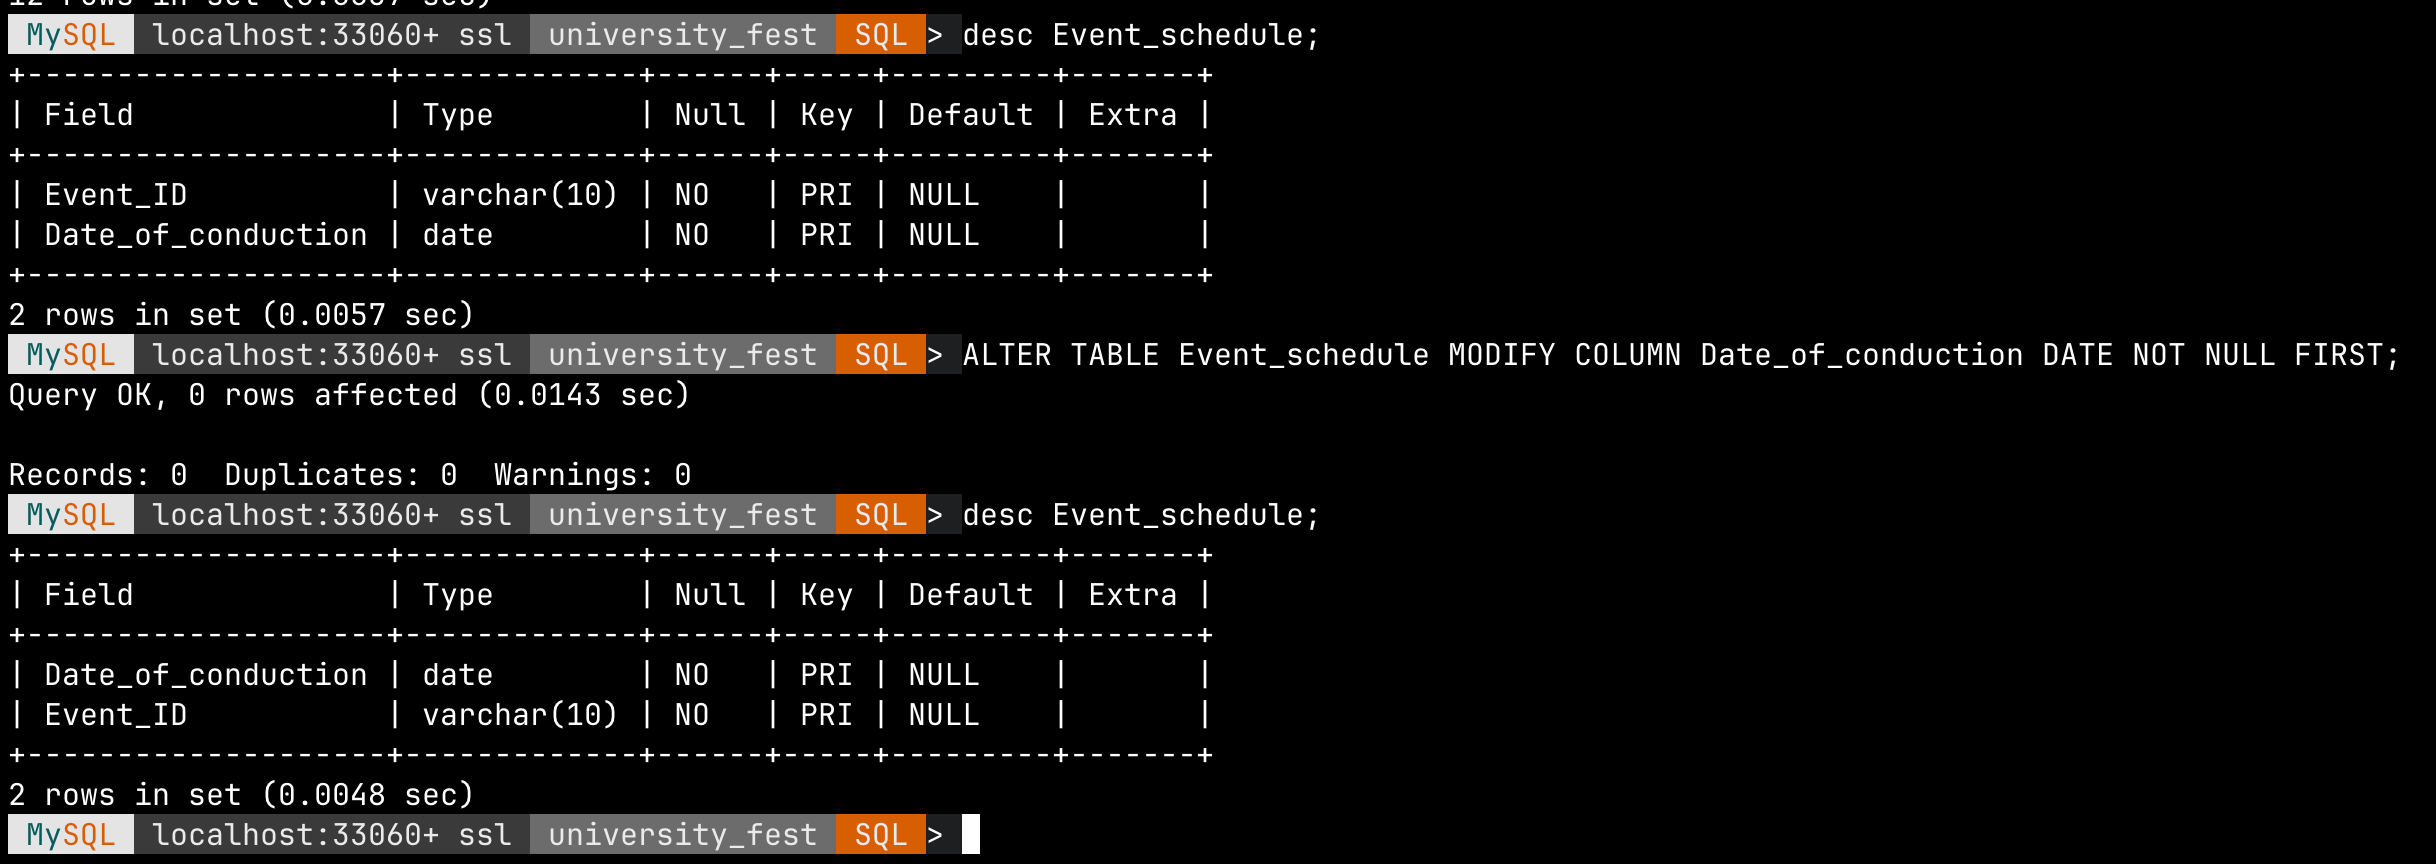
\includegraphics[width=0.7\linewidth]{images/task 2/5.png}
\end{figure}

\section{Task 3}

\begin{itemize}
    \item Which is the sql command to know the current database in MySQL? \\ 
\begin{lstlisting}[language=SQL]
SELECT DATABASE();
\end{lstlisting}  

    \item Which is the sql command to clear the command prompt window of MySQL? \\
    \begin{lstlisting}[language=SQL]
\c
OR 
CLEAR;
\end{lstlisting}
    \item Can you rename the database in MySQL? \\
    \begin{lstlisting}[language=SQL]
SELECT DATABASE();
\end{lstlisting}

    \item What is the command to remove a table along with its structure? \\
    \begin{lstlisting}[language=SQL]
DROP TABLE table_name;
\end{lstlisting}

    \item Specify the difference between drop table and truncate table? \\
    \begin{itemize}
        \item \texttt{DROP TABLE}: Removes the entire table structure and all data permanently. The table definition is also deleted.
        \item \texttt{TRUNCATE TABLE}: Removes only the data from the table but keeps the table structure intact. It's faster than DELETE but cannot be rolled back.
    \end{itemize}

    \item Can a table have more than one primary key? \\

    A table can have only a single primary key, but the primary key can be a composite of multiple attributes (\textit{composite primary key})
    
    \item Can a foreign key value be null? \\

Yes, foreign key values can be \texttt{NULL} unless explicitly constrained with \texttt{NOT NULL}
    
    \item Can a primary key value be null? Which constraint is this? \\

No, primary key values cannot be \texttt{NULL}
    
    \item Upon describing the table using the command “desc tablename” what information about the table is given. \\

The information about the table upon describing the table is as follows
\begin{itemize}
    \item Field
    \item Type
    \item Null
    \item Key
    \item Default
    \item Extra
\end{itemize}
    
    \item Can a primary key for a table be changed? If yes how? \\

    \begin{enumerate}
        \item First drop the existing primary key: \texttt{ALTER TABLE table\_name DROP PRIMARY KEY};
        \item Then add the new primary key: \texttt{ALTER TABLE table\_name ADD PRIMARY KEY (new\_column);}
    \end{enumerate}

\end{itemize}

% \begin{figure}[H]
%     \centering
%     \makebox[\textwidth][c]{
%         \includegraphics[width=1.1\linewidth]{Airport.drawio.png}
%     }
%     \caption{ER Diagram for an Airport Management System}
%     \label{fig:ermodel}
% \end{figure}

% \newpage

% \section{Relational Schema}

% \begin{figure}[H]
%     \centering
%     \makebox[\textwidth][c]{
%         \includegraphics[width=1.1\linewidth]{Relational_Schema_AMS.drawio.png}
%     }
%     \caption{Relational Schema}
%     \label{fig:relschema}
% \end{figure}

\end{document}
